\documentclass[aspectratio=43]{beamer}
% Theme works only with a 4:3 aspect ratio
\usetheme{CSCS}

\usepackage{tikz}
\usepackage{pgfplots}
\usepackage{pgfplotstable}
\usetikzlibrary{pgfplots.groupplots,spy,patterns}
\usetikzlibrary{arrows.meta}
\usetikzlibrary{positioning}
\usepackage{listings}
\usepackage{color}
\usepackage{tcolorbox}
\usepackage{anyfontsize}
\usepackage{xspace}
\usepackage{graphicx}
\usepackage{pifont}

% define footer text
\newcommand{\footlinetext}{Alps User Environments}

% Select the image for the title page
\newcommand{\picturetitle}{slide-images/image5.pdf}

% fonts for maths
\usefonttheme{professionalfonts}
\usefonttheme{serif}

% source code listing
\newcommand\TS{\rule{0pt}{2.6ex}}       % Top strut
\newcommand\BS{\rule[-1.2ex]{0pt}{0pt}} % Bottom strut
\newcommand{\hl}[1]{\textbf{\textcolor{blue}{#1}}} % for hilighting optimal entries in tables
\newcommand{\rl}[1]{\textbf{\textcolor{red}{#1}}} % for hilighting sub-optimal entries in tables
\newcommand{\img}[1]{{\Large \textbf{IMAGE {#1}}}}
\newcommand{\hilight}[1]{\textcolor{blue!20!orange}{#1}}
\newcommand{\alps}[0]{Alps\xspace}
\newcommand{\stackinator}[0]{Stackinator\xspace}

% set indent to a more reasonable level (so that itemize can be used in columns)
\setlength{\leftmargini}{20pt}

\DeclareTextFontCommand{\emph}{\color{blue!85!black}}

\author{
    \textbf{B.~Cumming},
    J.~Coles,
    T-I.~Manitaras,
    J-G.~Piccinali,
    S.~Pintarelli,
    H.~Stoppels}
\title{\centering Deploying Alternative User Environments on Alps}
\subtitle{CUG23 -- Helsinki}

\begin{document}

\setlength\labelsep   {\dimexpr\labelsep - 0.2em\relax}
\setlength\leftmargini{\dimexpr\leftmargini - 1.0em\relax}

% TITLE SLIDE
\cscstitle

\cscschapter{Setting the scene: motivation}

%-------------------------------------------
\begin{frame}[fragile]{Alps}
    Alps is the new Cray EX-based system at CSCS.

    \vspace{20pt}

    Borrow slide from Maxime's presentation showing the different vClusters

    \vspace{20pt}

    Consolidate disparate clusters onto a single Cray EX system

    \vspace{20pt}

    using CSM underneath -- each vCluster is depoloyed with its own software environment, scheduler, storage and network isolation

\end{frame}
%-------------------------------------------

%-------------------------------------------
\begin{frame}[fragile]{Monolithic Software Stacks}
    \begin{columns}[T]
        \begin{column}{0.5\textwidth}
            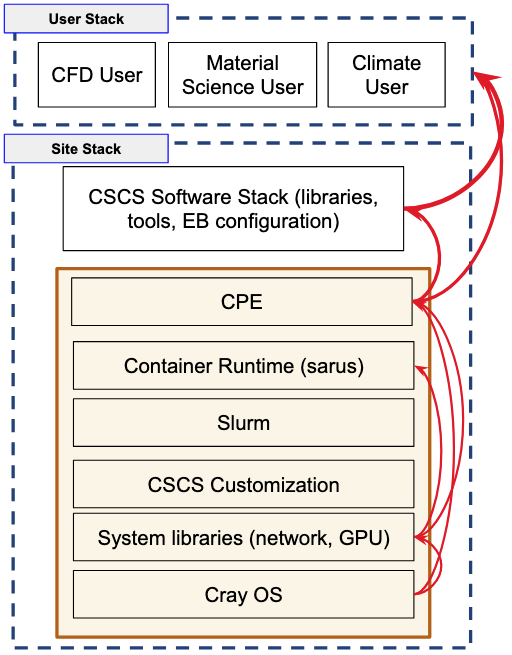
\includegraphics[width=\textwidth]{images/stack-old.png}
        \end{column}
        \begin{column}{0.5\textwidth}

            \small

            Sites build software for users using compilers and libraries from CPE
            % point out presentations past and present
            \begin{itemize}
                \item install all the software for all the users on a shared file system.
                \item modules alongside CPE modules
            \end{itemize}

            Is CPE a solid foundation when:
            \begin{itemize}
                \item it changes every 3 months
                \item it exposes a large surface area
                \item bugs will take 3-6 months minimum for fixes to be available
            \end{itemize}
        \end{column}
    \end{columns}
\end{frame}
%-------------------------------------------

%-------------------------------------------
\begin{frame}[fragile]{Bespoke SW stacks}
    \begin{columns}[T]
        \begin{column}{0.5\textwidth}

            Build use case and workflow specific software stacks:
            \begin{itemize}
                \item only packages that are needed
                \item deployed independently of one-another
                \item deployed independently of one-another
            \end{itemize}

            Build them on a simple foundation:
            \begin{itemize}
                \item CrayOS + libfabric + Slurm + xpmemm
                \item \emph{no CPE}
                \item infrequent changes
                \item small surface area
            \end{itemize}


        \end{column}
        \begin{column}{0.5\textwidth}
            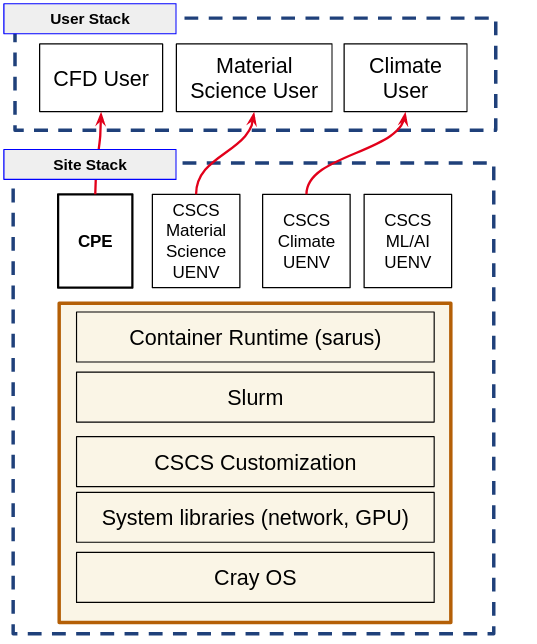
\includegraphics[width=\textwidth]{images/stack-new.png}
        \end{column}
    \end{columns}
\end{frame}
%-------------------------------------------

%-------------------------------------------
\begin{frame}[fragile]{Objectives}
    Software environments have the following objectives that make them DevOps compatible:
    \begin{itemize}
        \item reproducable from simple recipes
        \item versionable with git
        \item support easy roll back
        \item adapt to changes in the underlying system without modifying the recipe
        \item testable
    \end{itemize}
\end{frame}
%-------------------------------------------

\cscschapter{The stackinator: building environments}

\cscschapter{Deploying spack-stacks}

\cscschapter{Results}

\cscschapter{Wrapping up}

%-------------------------------------------
\begin{frame}[fragile]{Template}
    hello
    \begin{itemize}
        \item world
    \end{itemize}
\end{frame}
%-------------------------------------------

%-------------------------------------------
\begin{frame}[fragile]{Dual Column Example}
    \begin{columns}[T]
        \begin{column}{0.5\textwidth}
            %\includegraphics[width=\textwidth]{images/ls_term.png}
            Graphics

            \vspace{10pt}

            \begin{lstlisting}[style=arblang]
(restrict (terminal) (tag 3))
            \end{lstlisting}

            The tips (terminals) of the dendritic arbor (tag 3).

        \end{column}
        \begin{column}{0.5\textwidth}
            graphics!
            %\includegraphics[width=\textwidth]{images/reg_radle5.png}

            \vspace{10pt}

            \begin{lstlisting}[style=arblang]
(radius_le (all) 0.5)
            \end{lstlisting}
            All parts of the cell with radius less than or equal to 0.5 $\mu$m.

        \end{column}
    \end{columns}
\end{frame}
%-------------------------------------------

%-------------------------------------------
\begin{frame}[fragile]{Python code example}
    \begin{lstlisting}[style=talkpython]
import arbor as arb

# Create a cable_cell description
labels = {...}
morph = arb.swc_import('purkinje.swc')
cell = arb.cable_cell(morph, labels)
    \end{lstlisting}
\end{frame}
%-------------------------------------------

\cscschapter{A chapter}


\end{document}
